\documentclass[a4paper]{article}

\usepackage[english]{babel}
\usepackage[utf8]{inputenc}
\usepackage{graphicx}
\usepackage{enumitem}

\graphicspath{ {./images/} }
\setlength\parindent{0pt}
    
\title{CE2210, Sec. B \\Homework 6}
\author{Evan Wilcox}
\date{Due May 8, 2019}
    
\begin{document}
    \maketitle

    \begin{enumerate}
      %1
      \item  
      \begin{enumerate}

        \item Boolean Equations \\
        
        $f(t) = \overline{p(t) \cdot A(t)}$ \\
        $D_{A}(t) = p(t) \cdot A(t)$ \\



        \item State Table \\
        
        \begin{tabular}{ c c | c | c } 
        Input & State & Output & Next State \\ 
        $p(t)$ & $A(t)$ & $f(t)$ & $A(t+1)$ \\ \hline
        0 & 0 & 1 & 0 \\
        0 & 1 & 1 & 0 \\
        1 & 0 & 1 & 0 \\
        1 & 1 & 0 & 1 \\
        \end{tabular}


        \vspace{0.5cm}
        \item State Diagram \\
        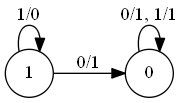
\includegraphics[scale=0.5]{1c}


      \end{enumerate}

      \vspace{0.75cm}
      %2
      \item  
      \begin{enumerate}

        \item State Table \\
        
        \begin{tabular}{ c c | c | c } 
          Input & State & Output & Next State \\ 
          $c(t)$ & $X(t)$ & $T(t)$ & $X(t+1)$ \\ \hline
          0 & 0 & 0 & 0 \\
          0 & 1 & 1 & 1 \\
          1 & 0 & 1 & 1 \\
          1 & 1 & 1 & 1 \\
          \end{tabular}

        \vspace{0.5cm}
        \item State Diagram \\
        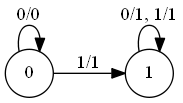
\includegraphics[scale=0.5]{2b}

      \end{enumerate}

      \newpage
      %3
      \item State Diagram \\
      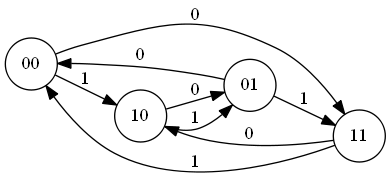
\includegraphics[scale=0.5]{3}

      \vspace{1cm}
      %4
      \item 
      \begin{enumerate}
        
        \item State Table \\
        
        \begin{tabular}{ccc|c}
          \multicolumn{2}{c}{Inputs} & State & Next State \\
          $d_{1}(t)$ & $d_{0}(t)$ & $Q(t)$ & $Q(t+1)$ \\ \hline
          0 & 0 & 0 & 1 \\
          0 & 0 & 1 & 1 \\
          0 & 1 & 0 & 1 \\
          0 & 1 & 1 & 1 \\ \hline
          1 & 0 & 0 & 0 \\
          1 & 0 & 1 & 0 \\
          1 & 1 & 0 & 0 \\
          1 & 1 & 1 & 0 \\
         \end{tabular}

        \vspace{0.5cm}
        \item Circuit Diagram 
        \vspace{5cm}

      \end{enumerate}
    
      \newpage
      %5
      \item 
      \begin{enumerate}

        \item State Diagram \\
        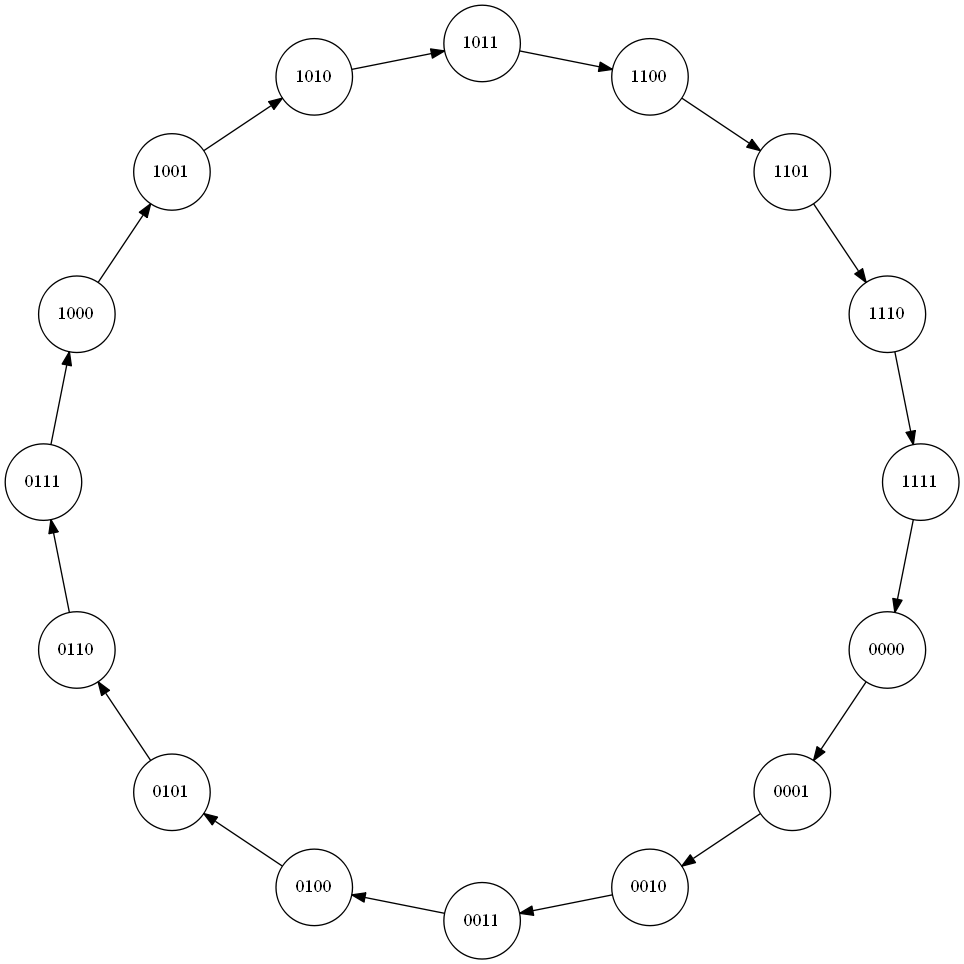
\includegraphics[scale=0.35]{5a}

        \item State Table \\
        
        \begin{tabular}{cccc|cccc}
          \multicolumn{4}{c}{States} & \multicolumn{4}{|c}{Next States} \\
          $A_{3}(t)$ & $A_{2}(t)$ & $A_{1}(t)$ & $A_{0}(t)$ & $A_{3}(t$+$1)$ & $A_{2}(t$+$1)$ & $A_{1}(t$+$1)$ & $A_{0}(t$+$1)$ \\ \hline
          0 & 0 & 0 & 0 & 0 & 0 & 0 & 1 \\
          0 & 0 & 0 & 1 & 0 & 0 & 1 & 0 \\
          0 & 0 & 1 & 0 & 0 & 0 & 1 & 1 \\
          0 & 0 & 1 & 1 & 0 & 1 & 0 & 0 \\ \hline
          0 & 1 & 0 & 0 & 0 & 1 & 0 & 1 \\
          0 & 1 & 0 & 1 & 0 & 1 & 1 & 0 \\
          0 & 1 & 1 & 0 & 0 & 1 & 1 & 1 \\
          0 & 1 & 1 & 1 & 1 & 0 & 0 & 0 \\ \hline
          1 & 0 & 0 & 0 & 1 & 0 & 0 & 1 \\
          1 & 0 & 0 & 1 & 1 & 0 & 1 & 0 \\
          1 & 0 & 1 & 0 & 1 & 0 & 1 & 1 \\
          1 & 0 & 1 & 1 & 1 & 1 & 0 & 0 \\ \hline
          1 & 1 & 0 & 0 & 1 & 1 & 0 & 1 \\
          1 & 1 & 0 & 1 & 1 & 1 & 1 & 0 \\
          1 & 1 & 1 & 0 & 1 & 1 & 1 & 1 \\
          1 & 1 & 1 & 1 & 0 & 0 & 0 & 0 \\
        \end{tabular}

        \newpage
        \item Boolean Equations \\
        
        $D_{3}(t) = A_{3}(t)\overline{A}_{2}(t) + A_{3}(t)\overline{A}_{1}(t) + A_{3}(t)\overline{A}_{0}(t) + \overline{A}_{3}(t)A_{2}(t)A_{1}(t)A_{0}(t)$ \\
        $D_{2}(t) = A_{2}(t)\overline{A}_{1}(t) + A_{2}(t)\overline{A}_{0}(t) + \overline{A}_{2}(t)A_{1}(t)A_{0}(t)$ \\
        $D_{1}(t) = A_{1}(t) \oplus A_{0}(t)$ \\
        $D_{0}(t) = \overline{A}_{0}(t)$ \\

        \item Circuit Diagram \\

      \end{enumerate}

      \newpage
      %6
      \item 
      \begin{enumerate}

        \item State Table \\

        \begin{tabular}{ccc|c|c}
          \multicolumn{2}{c}{Input} & State & Output & Next State \\
          $a(t)$ & $b(t)$ & $x(t)$ & $f(t)$ & $x(t+1)$ \\ \hline
          0 & 0 & 0 & 0 & 1 \\
          0 & 0 & 1 & 0 & 1 \\
          0 & 1 & 0 & 0 & 1 \\
          0 & 1 & 1 & 1 & 0 \\ \hline
          1 & 0 & 0 & 0 & 1 \\
          1 & 0 & 1 & 0 & 1 \\
          1 & 1 & 0 & 1 & 0 \\
          1 & 1 & 1 & 1 & 0
        \end{tabular}

        \vspace{0.5cm}
        \item State Diagram \\
        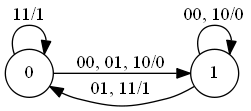
\includegraphics[scale=0.5]{6b}

      \end{enumerate}

      %7
      \item State Table \\
      
      \begin{tabular}{ ccc|cc|cc|cc }
        Input & \multicolumn{2}{c}{States} & \multicolumn{2}{c}{Outputs} & \multicolumn{2}{c}{Next States} & \multicolumn{2}{c}{TFF}\\
        $w(t)$ & $x(t)$ & $y(t)$ & $f_{x}(t)$ & $f_{y}(t)$ & $x(t+1)$ & $y(t+1)$ & $T_{x}(t)$ & $T_{y}(t)$ \\ \hline
        0 & 0 & 0 & 1 & 0 & 1 & 0 & 1 & 0\\
        0 & 0 & 1 & 1 & 0 & 1 & 0 & 1 & 1\\
        0 & 1 & 0 & 0 & 0 & 0 & 0 & 1 & 0\\
        0 & 1 & 1 & 0 & 0 & 0 & 0 & 1 & 1\\ \hline
        1 & 0 & 0 & 0 & 0 & 0 & 0 & 0 & 0\\
        1 & 0 & 1 & 0 & 0 & 0 & 0 & 0 & 1\\
        1 & 1 & 0 & 0 & 0 & 0 & 0 & 1 & 0\\
        1 & 1 & 1 & 0 & 1 & 0 & 1 & 1 & 0\\
      \end{tabular}

      \vspace{0.5cm}
      Boolean Equations \\

      $f_{x}(t) = \overline{w}(t)\overline{x}(t)$ \\
      $f_{y}(t) = w(t)x(t)y(t)$ \\
      $T_{x}(t) = \overline{w}(t) + x(t)$ \\
      $T_{y}(t) = \overline{w}(t)y(t) + \overline{x}(t)y(t)$ \\

      \vspace{1cm}
      Circuit Diagram on back of this page.


    \end{enumerate}

\end{document}